\chapter{Les sons autour de nous}\label{ch:g3:sound-around-us}

Fredonne ta chanson préférée --- et, pendant que tu fredonnes, pose
doucement deux doigts sur le devant de ta gorge. Tu sens ce
tremblement~? Tu viens de toucher un \omterm{def:g3:sound-around-us:sound}{son} sur son lieu de naissance.
Chaque voix, chaque tambour, chaque porte qui grince fabrique son son
exactement de la même façon, et ce chapitre part à la chasse au truc.

\section{Où naissent les sons}

\begin{definition}[Vibration]\label{def:g3:sound-around-us:vibration}
Une \emph{vibration}\index{vibration} est un tremblement très
rapide --- un mouvement de va-et-vient répété de nombreuses fois par
seconde, souvent trop vite pour que l'œil le suive. Une corde de
guitare pincée vibre~: tu ne vois qu'un flou, mais le bout de ton
doigt sent le bourdonnement.
\end{definition}

\begin{definition}[Son]\label{def:g3:sound-around-us:sound}
Un \emph{son}\index{son} est ce que nous entendons quand un objet
vibre et que son tremblement voyage dans l'\omterm{def:g2:air-around-us:air}{air} jusqu'à nos oreilles.
L'objet qui vibre est la \emph{source} du son --- une corde, une peau
de tambour, une cloche, ta propre gorge.
\end{definition}

\begin{method}[Faire danser le riz]\label{met:g3:sound-around-us:rice}
Pour \emph{voir} naître un \omterm{def:g3:sound-around-us:sound}{son}~:
\begin{enumerate}
  \item éparpiller quelques grains de riz sur la peau d'un tambour
        (ou sur le couvercle en plastique d'une boîte, ou sur une
        peau de ballon tendue)~;
  \item frapper la peau près des grains --- boum~: les grains
        sautent~!
  \item maintenant, se contenter de \emph{crier} vers la peau, de
        tout près~: les grains tremblent de nouveau, sans être
        touchés.
\end{enumerate}
La peau vibre chaque fois qu'elle sonne --- et même un \omterm{def:g3:sound-around-us:sound}{son} venu de ta
bouche la fait trembler.
\end{method}

\begin{omfigure}
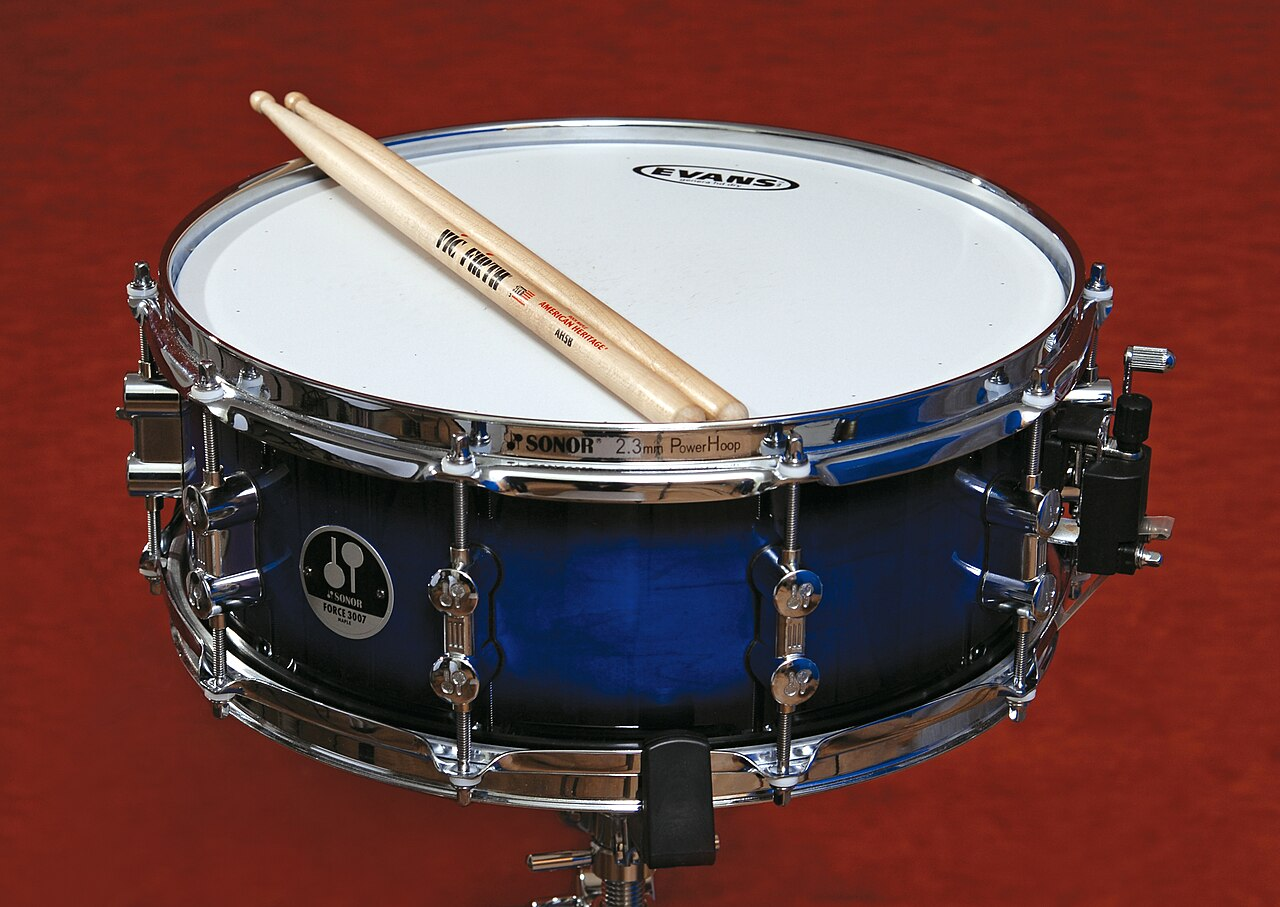
\includegraphics[width=0.58\linewidth]{images/book1/drum.jpg}

{\small Un vrai tambour pour l'expérience du riz~: la peau blanche
est la partie qui tremble. Éparpille quelques grains dessus, frappe à
côté d'eux --- une peau qui sonne est une peau qui tremble, et le riz
danse pour le prouver. \emph{Photo~: Vladimir Morozov, CC BY 2.0.}}
\end{omfigure}

\begin{proposition}[Pas de vibration, pas de son]\label{prop:g3:sound-around-us:novib}
Tout son vient d'une \omterm{def:g3:sound-around-us:vibration}{vibration} --- et quand la \omterm{def:g3:sound-around-us:vibration}{vibration} s'arrête, le
\omterm{def:g3:sound-around-us:sound}{son} s'arrête avec elle, instantanément. Frappe une cymbale et
laisse-la résonner~; puis saisis-la fermement à deux mains~: le
silence, à l'instant même où ta poigne arrête le tremblement.
\end{proposition}

\begin{example}[Des sources de son partout]\label{ex:g3:sound-around-us:sources}
Pars à la chasse à la \omterm{def:g3:sound-around-us:vibration}{vibration} derrière chaque son~: la guitare ---
les cordes pincées tremblent~; le tambour --- la peau frappée
tremble~; ta voix --- deux petits replis de ta gorge tremblent quand
l'\omterm{def:g2:air-around-us:air}{air} de tes poumons file entre eux (c'est le bourdonnement que tes
doigts ont senti)~; la mouche qui bourdonne --- ses ailes tremblent
des centaines de fois par seconde~; la porte claquée --- toute la
porte et son cadre frémissent un instant.
\end{example}

\section{Fort et faible, aigu et grave}

\begin{example}[Fort, c'est un grand
tremblement]\label{ex:g3:sound-around-us:loud}
Pince doucement un élastique tendu~: un petit flou, un \omterm{def:g3:sound-around-us:sound}{son} faible.
Pince-le fort~: un large flou, un \omterm{def:g3:sound-around-us:sound}{son} fort. Plus la source tremble
fort --- plus son va-et-vient est ample --- plus le \omterm{def:g3:sound-around-us:sound}{son} est
\emph{fort}. Observe aussi les grains de riz~: une petite tape les
fait frissonner, un boum puissant les projette en l'\omterm{def:g2:air-around-us:air}{air}.
\end{example}

\begin{example}[Aigu et grave]\label{ex:g3:sound-around-us:pitch}
Tends un élastique sur une boîte ouverte et pince-le~; puis pince-le
en son milieu et fais vibrer la moitié la plus courte~: le \omterm{def:g3:sound-around-us:sound}{son}
devient plus \emph{aigu}, comme un pépiement d'oiseau. Ce qui est
court, tendu et fin tremble plus vite et chante aigu~; ce qui est
long, lâche et épais tremble plus lentement et chante grave. Voilà
pourquoi la petite flûte pépie et le gros tuba gronde --- et pourquoi
la corde la plus fine de la guitare est celle qui chante le plus
aigu.
\end{example}

\begin{omfigure}
\begin{tikzpicture}[scale=0.85]
  % whole band, stretched over the open box, vibrating end to end
  \draw[thick] (0.3,0) rectangle (4.9,1.1);
  \draw[omDef, very thick] (0.3,1.1) -- (4.9,1.1);
  \draw[dashed, omDef] (0.3,1.1) .. controls (2.6,1.62) .. (4.9,1.1);
  \draw[dashed, omDef] (0.3,1.1) .. controls (2.6,0.58) .. (4.9,1.1);
  \node[below, font=\small, align=center] at (2.6,-0.3)
    {élastique entier~:\\tremblement lent, son grave};
  % pinched at the middle: only the short half vibrates
  \draw[thick] (6.5,0) rectangle (11.1,1.1);
  \draw[omDef, very thick] (6.5,1.1) -- (11.1,1.1);
  \fill[omExo] (8.8,1.1) circle (0.1);
  \node[above, font=\footnotesize, omExo] at (8.8,1.32) {pincement};
  \draw[dashed, omDef] (8.8,1.1) .. controls (9.95,1.45) .. (11.1,1.1);
  \draw[dashed, omDef] (8.8,1.1) .. controls (9.95,0.75) .. (11.1,1.1);
  \node[below, font=\small, align=center] at (8.8,-0.3)
    {moitié courte~:\\tremblement rapide, son aigu};
\end{tikzpicture}

{\small La guitare en élastique~: l'élastique entier oscille le plus
largement en son milieu, retenu à ses deux bouts, et chante grave~;
la moitié pincée, plus courte, tremble plus vite et chante plus
aigu.}
\end{omfigure}

\begin{remark}[Protège le petit tambour de ton
oreille]\label{rem:g3:sound-around-us:ears}
Au fond de ton oreille, une minuscule peau --- plus fine que du
papier --- tremble à chaque son qui arrive, exactement comme le
tambour aux grains de riz. Les \omterm{def:g3:sound-around-us:sound}{sons} trop forts la secouent trop
violemment~: une musique très forte, des machines, des feux
d'artifice peuvent l'abîmer pour toujours, et elle ne repousse pas.
Bouche-toi les oreilles près d'un bruit fort, et ne crie jamais dans
l'oreille de quelqu'un --- les oreilles n'ont pas de paupières.
\end{remark}

\section{De la source à l'oreille}

\begin{example}[Le voyage d'un applaudissement]\label{ex:g3:sound-around-us:journey}
Un camarade tape dans ses mains à l'autre bout de la cour. Le claquement
fait trembler l'\omterm{def:g2:air-around-us:air}{air}~; le tremblement s'étale dans l'\omterm{def:g2:air-around-us:air}{air} dans toutes
les directions, comme les ronds autour d'un caillou jeté dans un
étang~; une partie atteint ton oreille et fait trembler sa petite
peau --- et tu entends le claquement. Source, voyage, oreille~: tous
les \omterm{def:g3:sound-around-us:sound}{sons} que tu as entendus dans ta vie ont fait ce trajet. À quelle
vitesse se fait le voyage, et qu'est-ce qu'il peut traverser~? Le
chapitre sur le \omterm{def:g3:sound-around-us:sound}{son} de l'an prochain s'attaque exactement à ces
questions.
\end{example}

\section{Exercices}

\begin{exercise}[$\star$]\label{exo:g3:sound-around-us:1}
Qu'est-ce qu'une \omterm{def:g3:sound-around-us:vibration}{vibration}~? Nomme la partie qui vibre dans~: une
guitare~; \ un tambour~; \ ta voix~; \ une mouche qui bourdonne.
\end{exercise}

\begin{exercise}[$\star$]\label{exo:g3:sound-around-us:2}
Dans l'expérience du riz, que prouvent les grains qui sautent au
sujet d'une peau de tambour qui sonne~?
\end{exercise}

\begin{exercise}[$\star$]\label{exo:g3:sound-around-us:3}
Pourquoi saisir une cymbale qui résonne la fait-il taire aussitôt~?
Quelle loi du chapitre est à l'œuvre~?
\end{exercise}

\begin{exercise}[$\star$]\label{exo:g3:sound-around-us:4}
Pour que l'élastique sonne plus \emph{fort}, que changes-tu à ton
pincement~? À quoi ressemble alors le flou de l'élastique~?
\end{exercise}

\begin{exercise}[$\star$]\label{exo:g3:sound-around-us:5}
Qu'est-ce qui chante le plus aigu~: la moitié courte pincée ou
l'élastique entier~? \ La petite flûte ou le gros tuba~? \ La corde la
plus fine ou la plus épaisse de la guitare~?
\end{exercise}

\begin{exercise}[$\star$]\label{exo:g3:sound-around-us:6}
Fredonne avec les doigts sur la gorge, puis arrête de fredonner. Que
sentent tes doigts, et à quel moment exactement la sensation
s'arrête-t-elle~?
\end{exercise}

\begin{exercise}[$\star$]\label{exo:g3:sound-around-us:7}
Raconte en trois étapes le voyage d'un claquement de mains, des mains
de ton camarade jusqu'à ton oreille.
\end{exercise}

\begin{exercise}[$\star$]\label{exo:g3:sound-around-us:8}
Pourquoi faut-il tenir les \omterm{def:g3:sound-around-us:sound}{sons} très forts loin des oreilles~? Quel
minuscule élément de l'oreille est en danger, et à quoi
ressemble-t-il, dans ce chapitre~?
\end{exercise}

\begin{exercise}[$\star$]\label{exo:g3:sound-around-us:9}
Le peigne d'une boîte à musique a des dents de longueurs différentes.
Quelles dents jouent les notes aiguës et lesquelles les notes
graves~? Réponds avec la règle de \cref{ex:g3:sound-around-us:pitch}.
\end{exercise}

\begin{exercise}[$\star\star$]\label{exo:g3:sound-around-us:10}
Verse de l'eau dans une bouteille en verre et souffle en travers du
goulot~: un hululement~! Ajoute de l'eau et souffle de nouveau~: le
hululement devient plus aigu. Qu'est-ce qui tremble pour produire ce
\omterm{def:g3:sound-around-us:sound}{son} --- le verre, l'eau, ou l'\omterm{def:g2:air-around-us:air}{air} à l'intérieur~? Sers-toi de la
règle «~court, donc aigu~» pour défendre ta réponse.
\end{exercise}

\begin{exercise}[$\star\star$]\label{exo:g3:sound-around-us:11}
Maya dit~: «~Quand la télévision est en sourdine, l'écran bouge
quand même --- le mouvement tout seul doit donc faire du \omterm{def:g3:sound-around-us:sound}{son}.~»
Sers-toi de \cref{def:g3:sound-around-us:sound} et de l'expérience du
riz pour expliquer quel genre de mouvement fabrique du \omterm{def:g3:sound-around-us:sound}{son}, et
pourquoi les images d'un écran n'en font aucun.
\end{exercise}
